\documentclass{article}
\usepackage{fancyhdr}
\usepackage{amsthm}
\usepackage{etoolbox}
\usepackage{verbatim}
\usepackage{enumerate}
\usepackage{amsmath}
\usepackage{algorithmicx}
\usepackage{algorithm}
\usepackage{algpseudocode}
\usepackage{amssymb}
\usepackage{tikz}
	
\pagestyle{fancy}
\title{Chapter 18}
\author{Michelle Bodnar, Andrew Lohr}

\newcounter{curnum}
\setcounter{curnum}{0}

\newtheorem{th1}{Exercise} 
\newcommand{\calH}{\mathcal{H}}
\newcommand{\calX}{\mathcal{X}}
\newcommand{\calA}{\mathcal{A}}
\newcommand{\calY}{\mathcal{Y}}

\begin{document}
\maketitle


\noindent\textbf{Exercise 18.1-1}\\
If we allow $t=0$, then, since we only know that internal nodes have to have at least $t-1$ keys, it may be the case that some internal nodes represent no keys, a bad situation indeed.\\

\noindent\textbf{Exercise 18.1-3}\\
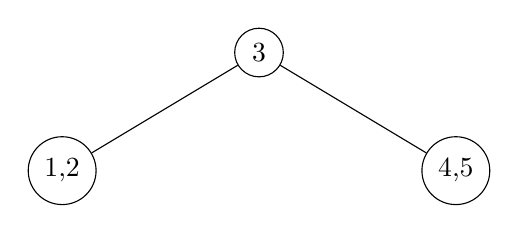
\begin{tikzpicture}[level/.style={sibling distance=50mm/#1}]
\node [circle,draw] (a){3}
  child {
  node [circle,draw] (b) {1,2}
  }
  child {
  node [circle,draw] (i) {4,5}
  };
\end{tikzpicture}

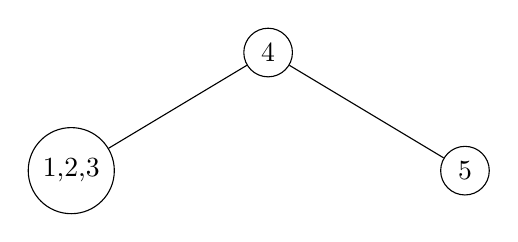
\begin{tikzpicture}[level/.style={sibling distance=50mm/#1}]
\node [circle,draw] (a){4}
  child {
  node [circle,draw] (b) {1,2,3}
  }
  child {
  node [circle,draw] (i) {5}
  };
\end{tikzpicture}

\begin{tikzpicture}[level/.style={sibling distance=50mm/#1}]
\node [circle,draw] (a){4}
  child {
  node [circle,draw] (b) {2}
  child {
  node [circle,draw] (c) {1}
  }
  child {
  node [circle,draw] (d) {3}
  }
  }
  child {
  node [circle,draw] (i) {5}
  };
\end{tikzpicture}

\begin{tikzpicture}[level/.style={sibling distance=50mm/#1}]
\node [circle,draw] (a){2}
  child {
  node [circle,draw] (b) {1}
  }
  child {
  node [circle,draw] (i) {4}
  child{
    node [circle,draw] (c) {3}
}
  child{  node [circle,draw] (d) {5}
}
    };
\end{tikzpicture}

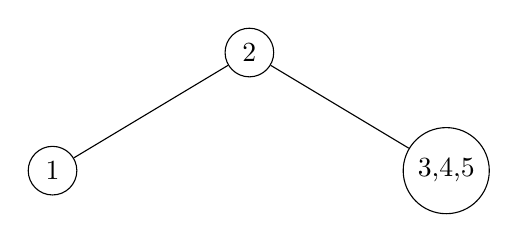
\begin{tikzpicture}[level/.style={sibling distance=50mm/#1}]
\node [circle,draw] (a){2}
  child {
  node [circle,draw] (b) {1}
  }
  child {
  node [circle,draw] (i) {3,4,5}
  };
\end{tikzpicture}

\begin{tikzpicture}[level/.style={sibling distance=50mm/#1}]
\node [circle,draw] (a){2,4}
  child {
  node [circle,draw] (b) {1}
  }
  child {
  node [circle,draw] (i) {3}
  }
    child {
  node [circle,draw] (i) {5}
  };
\end{tikzpicture}

\noindent\textbf{Exercise 18.1-5}\\
We would get a t=2 B-tree. It would have one, two, or three keys depending on if it has zero, one, or two red children respectively. Suppose that the left child is red, then it's keys becomes the first one, and that red node's children become the first and second children of the new node. Similarly, if it is the right child that is red, that key becomes the last key listed with the new node, and the red nodes children become the second to last and last children of the new node.\\

\noindent\textbf{Exercise 18.2-1}\\%should check

\begin{tikzpicture}[level/.style={sibling distance=50mm/#1}]
\node [circle,draw] (a){F}
  ;
\end{tikzpicture}


\begin{tikzpicture}[level/.style={sibling distance=50mm/#1}]
\node [circle,draw] (a){FS}
;
\end{tikzpicture}


\begin{tikzpicture}[level/.style={sibling distance=50mm/#1}]
\node [circle,draw] (a){FQS}
;
\end{tikzpicture}

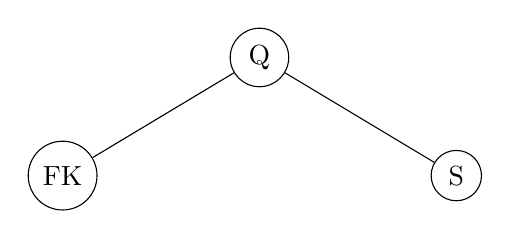
\begin{tikzpicture}[level/.style={sibling distance=50mm/#1}]
\node [circle,draw] (a){Q}
  child {
  node [circle,draw] (b) {FK}
  }
  child {
  node [circle,draw] (i) {S}
  };
\end{tikzpicture}

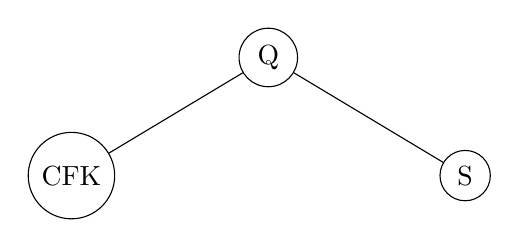
\begin{tikzpicture}[level/.style={sibling distance=50mm/#1}]
\node [circle,draw] (a){Q}
  child {
  node [circle,draw] (b) {CFK}
  }
  child {
  node [circle,draw] (i) {S}
  };
\end{tikzpicture}

\begin{tikzpicture}[level/.style={sibling distance=50mm/#1}]
\node [circle,draw] (a){FQ}
  child {
  node [circle,draw] (b) {C}
  }
  child{
  node[circle,draw] (c){KL}
  }
  child {
  node [circle,draw] (i) {S}
  };
\end{tikzpicture}

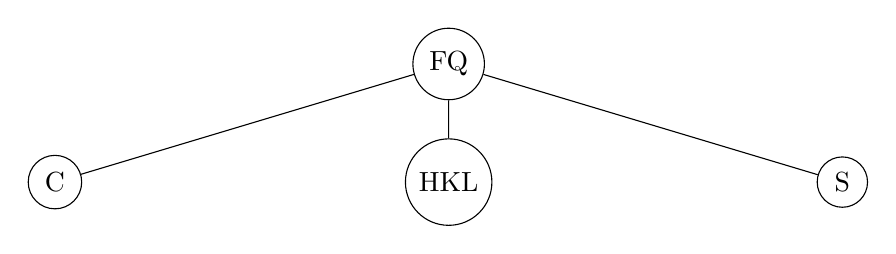
\begin{tikzpicture}[level/.style={sibling distance=50mm/#1}]
\node [circle,draw] (a){FQ}
  child {
  node [circle,draw] (b) {C}
  }
  child{
  node[circle,draw] (c){HKL}
  }
  child {
  node [circle,draw] (i) {S}
  };
\end{tikzpicture}

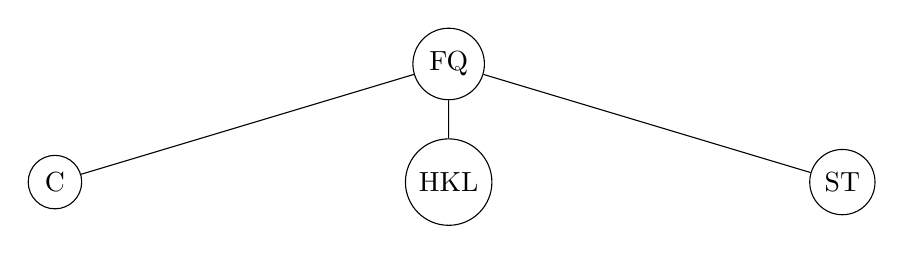
\begin{tikzpicture}[level/.style={sibling distance=50mm/#1}]
\node [circle,draw] (a){FQ}
  child {
  node [circle,draw] (b) {C}
  }
  child{
  node[circle,draw] (c){HKL}
  }
  child {
  node [circle,draw] (i) {ST}
  };
\end{tikzpicture}

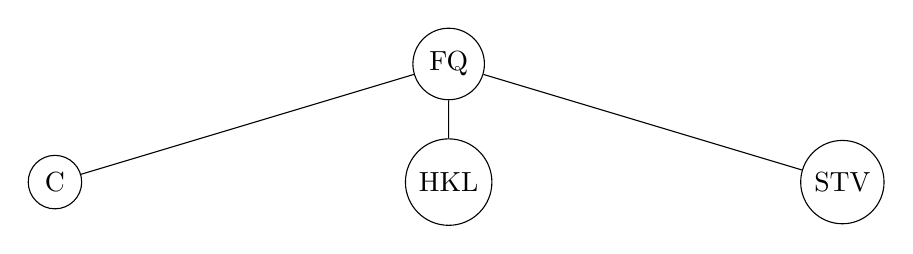
\begin{tikzpicture}[level/.style={sibling distance=50mm/#1}]
\node [circle,draw] (a){FQ}
  child {
  node [circle,draw] (b) {C}
  }
  child{
  node[circle,draw] (c){HKL}
  }
  child {
  node [circle,draw] (i) {STV}
  };
\end{tikzpicture}

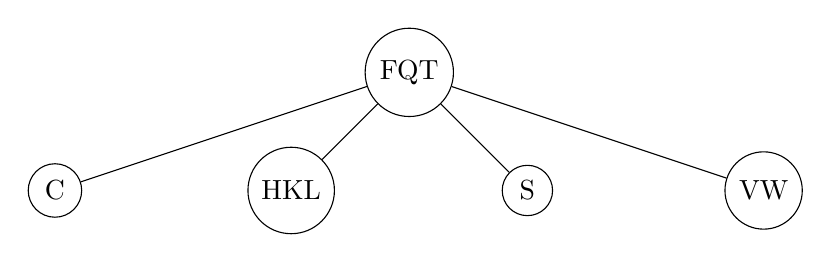
\begin{tikzpicture}[level/.style={sibling distance=30mm/#1}]
\node [circle,draw] (a){FQT}
  child {
  node [circle,draw] (b) {C}
  }
  child{
  node[circle,draw] (c){HKL}
  }
  child {
  node [circle,draw] (i) {S}
  }  child {
  node [circle,draw] (d) {VW}
  };
\end{tikzpicture}

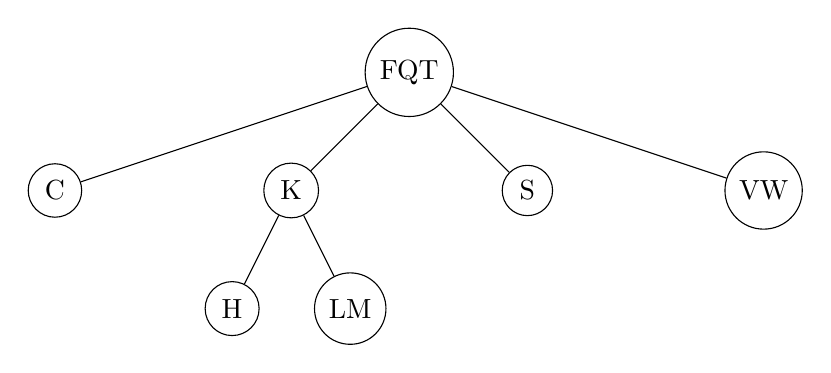
\begin{tikzpicture}[level/.style={sibling distance=30mm/#1}]
\node [circle,draw] (a){FQT}
  child {
  node [circle,draw] (b) {C}
  }
  child{
  node[circle,draw] (c){K}
  child{
  node[circle,draw] (e){H}
  }
  child{
  node[circle,draw] (f){LM}
    }
  }
  child {
  node [circle,draw] (i) {S}
  }  child {
  node [circle,draw] (d) {VW}
  };
\end{tikzpicture}

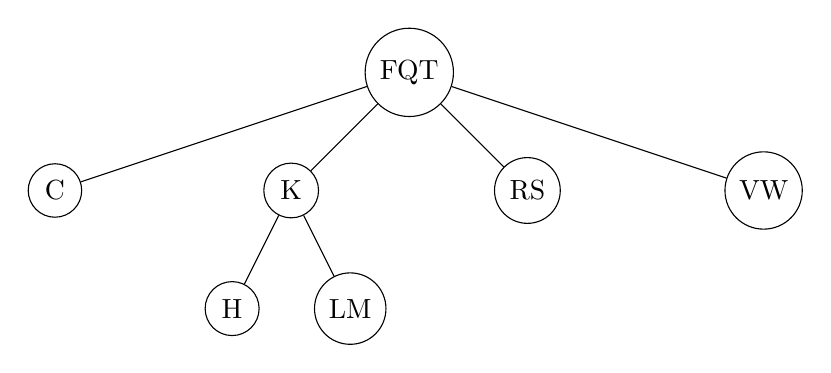
\begin{tikzpicture}[level/.style={sibling distance=30mm/#1}]
\node [circle,draw] (a){FQT}
  child {
  node [circle,draw] (b) {C}
  }
  child{
  node[circle,draw] (c){K}
  child{
  node[circle,draw] (e){H}
  }
  child{
  node[circle,draw] (f){LM}
    }
  }
  child {
  node [circle,draw] (i) {RS}
  }  child {
  node [circle,draw] (d) {VW}
  };
\end{tikzpicture}

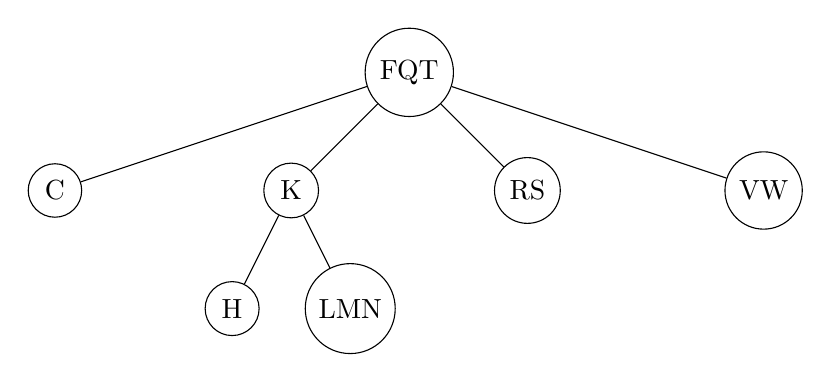
\begin{tikzpicture}[level/.style={sibling distance=30mm/#1}]
\node [circle,draw] (a){FQT}
  child {
  node [circle,draw] (b) {C}
  }
  child{
  node[circle,draw] (c){K}
  child{
  node[circle,draw] (e){H}
  }
  child{
  node[circle,draw] (f){LMN}
    }
  }
  child {
  node [circle,draw] (i) {RS}
  }  child {
  node [circle,draw] (d) {VW}
  };
\end{tikzpicture}

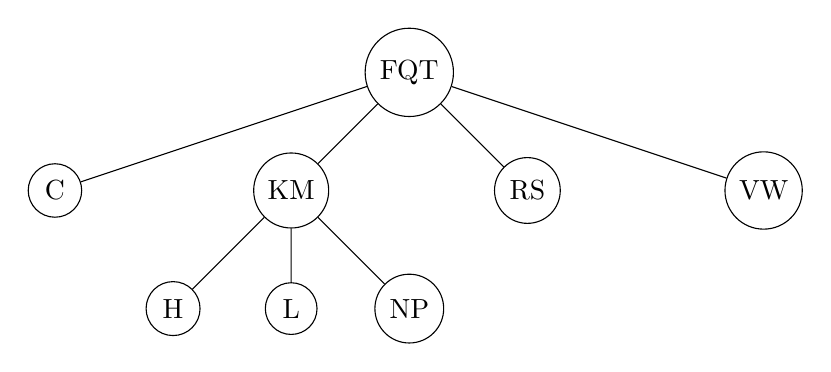
\begin{tikzpicture}[level/.style={sibling distance=30mm/#1}]
\node [circle,draw] (a){FQT}
  child {
  node [circle,draw] (b) {C}
  }
  child{
  node[circle,draw] (c){KM}
  child{
  node[circle,draw] (e){H}
  }
  child{
  node[circle,draw] (f){L}
    }
  child{
  node[circle,draw] (g){NP}
    }
    }
  child {
  node [circle,draw] (i) {RS}
  }  child {
  node [circle,draw] (d) {VW}
  };
\end{tikzpicture}

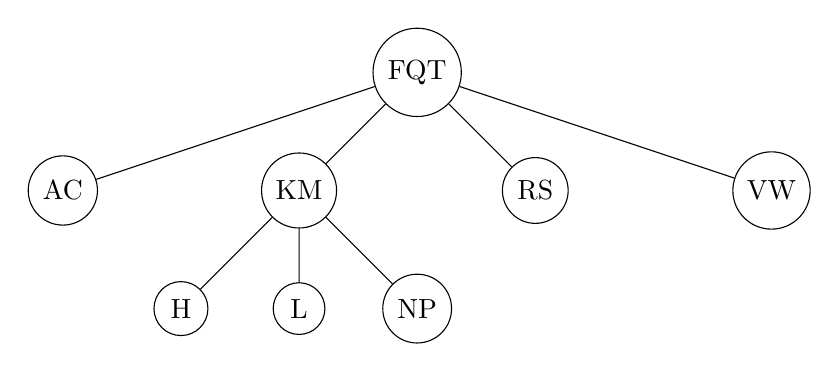
\begin{tikzpicture}[level/.style={sibling distance=30mm/#1}]
\node [circle,draw] (a){FQT}
  child {
  node [circle,draw] (b) {AC}
  }
  child{
  node[circle,draw] (c){KM}
  child{
  node[circle,draw] (e){H}
  }
  child{
  node[circle,draw] (f){L}
    }
  child{
  node[circle,draw] (g){NP}
    }
    }
  child {
  node [circle,draw] (i) {RS}
  }  child {
  node [circle,draw] (d) {VW}
  };
\end{tikzpicture}

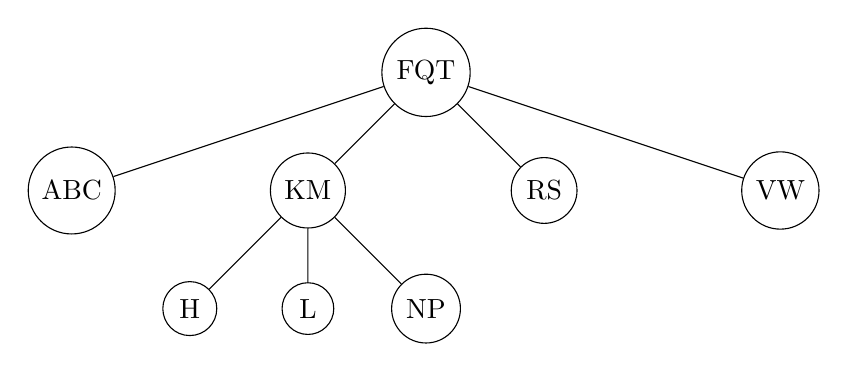
\begin{tikzpicture}[level/.style={sibling distance=30mm/#1}]
\node [circle,draw] (a){FQT}
  child {
  node [circle,draw] (b) {ABC}
  }
  child{
  node[circle,draw] (c){KM}
  child{
  node[circle,draw] (e){H}
  }
  child{
  node[circle,draw] (f){L}
    }
  child{
  node[circle,draw] (g){NP}
    }
    }
  child {
  node [circle,draw] (i) {RS}
  }  child {
  node [circle,draw] (d) {VW}
  };
\end{tikzpicture}

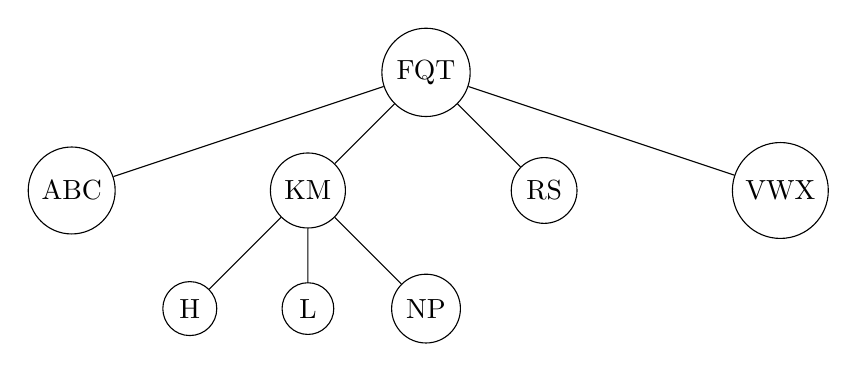
\begin{tikzpicture}[level/.style={sibling distance=30mm/#1}]
\node [circle,draw] (a){FQT}
  child {
  node [circle,draw] (b) {ABC}
  }
  child{
  node[circle,draw] (c){KM}
  child{
  node[circle,draw] (e){H}
  }
  child{
  node[circle,draw] (f){L}
    }
  child{
  node[circle,draw] (g){NP}
    }
    }
  child {
  node [circle,draw] (i) {RS}
  }  child {
  node [circle,draw] (d) {VWX}
  };
\end{tikzpicture}

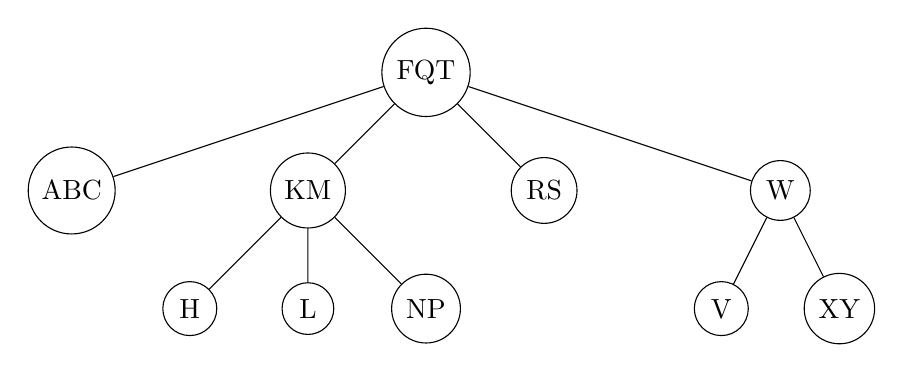
\begin{tikzpicture}[level/.style={sibling distance=30mm/#1}]
\node [circle,draw] (a){FQT}
  child {
  node [circle,draw] (b) {ABC}
  }
  child{
  node[circle,draw] (c){KM}
  child{
  node[circle,draw] (e){H}
  }
  child{
  node[circle,draw] (f){L}
    }
  child{
  node[circle,draw] (g){NP}
    }
    }
  child {
  node [circle,draw] (i) {RS}
  }  child {
  node [circle,draw] (d) {W}
  child{
  node [circle,draw] (h) {V}
  }
  child{
  node [circle,draw] (i) {XY}  
  }
  };
\end{tikzpicture}

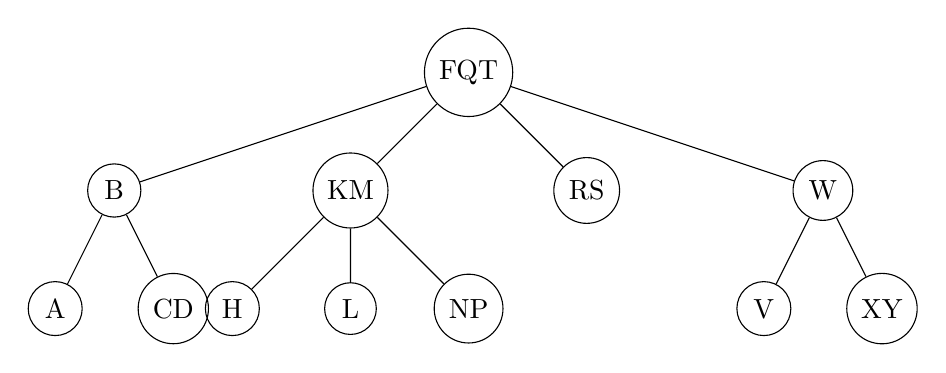
\begin{tikzpicture}[level/.style={sibling distance=30mm/#1}]
\node [circle,draw] (a){FQT}
  child {
  node [circle,draw] (b) {B}
  child{
  node [circle,draw] (j) {A}
    }
  child{
  node [circle,draw] (k) {CD}
  }
  }
  child{
  node[circle,draw] (c){KM}
  child{
  node[circle,draw] (e){H}
  }
  child{
  node[circle,draw] (f){L}
    }
  child{
  node[circle,draw] (g){NP}
    }
    }
  child {
  node [circle,draw] (i) {RS}
  }  child {
  node [circle,draw] (d) {W}
  child{
  node [circle,draw] (h) {V}
  }
  child{
  node [circle,draw] (i) {XY}  
  }
  };
\end{tikzpicture}

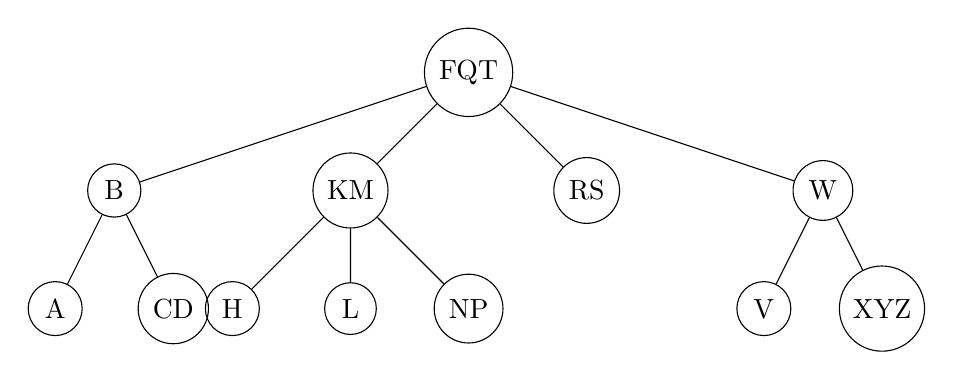
\begin{tikzpicture}[level/.style={sibling distance=30mm/#1}]
\node [circle,draw] (a){FQT}
  child {
  node [circle,draw] (b) {B}
  child{
  node [circle,draw] (j) {A}
    }
  child{
  node [circle,draw] (k) {CD}
  }
  }
  child{
  node[circle,draw] (c){KM}
  child{
  node[circle,draw] (e){H}
  }
  child{
  node[circle,draw] (f){L}
    }
  child{
  node[circle,draw] (g){NP}
    }
    }
  child {
  node [circle,draw] (i) {RS}
  }  child {
  node [circle,draw] (d) {W}
  child{
  node [circle,draw] (h) {V}
  }
  child{
  node [circle,draw] (i) {XYZ}  
  }
  };
\end{tikzpicture}

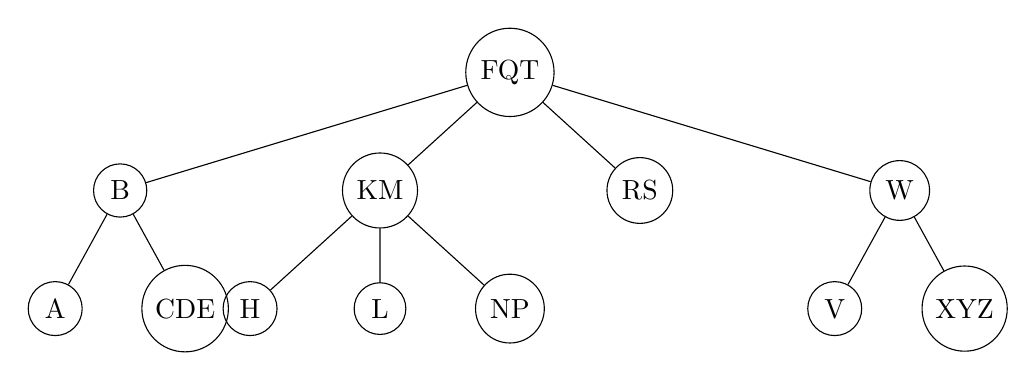
\begin{tikzpicture}[level/.style={sibling distance=33mm/#1}]
\node [circle,draw] (a){FQT}
  child {
  node [circle,draw] (b) {B}
  child{
  node [circle,draw] (j) {A}
    }
  child{
  node [circle,draw] (k) {CDE}
  }
  }
  child{
  node[circle,draw] (c){KM}
  child{
  node[circle,draw] (e){H}
  }
  child{
  node[circle,draw] (f){L}
    }
  child{
  node[circle,draw] (g){NP}
    }
    }
  child {
  node [circle,draw] (i) {RS}
  }  child {
  node [circle,draw] (d) {W}
  child{
  node [circle,draw] (h) {V}
  }
  child{
  node [circle,draw] (i) {XYZ}  
  }
  };
\end{tikzpicture}


\noindent\textbf{Exercise 18.2-3}\\
To find the minimum key, just always select the first child until you are on a leaf, then return the first key. To find the predecessor of a given key, fist find it. if it's on a leaf then just return the preceeding key. If it's not a leaf, then return the largest element(in an analogous way to finding minimum) of the child that immediately preceeds the key just found.\\ 

\noindent\textbf{Exercise 18.2-5}\\
You would modify the insertion procedure by, in B-TREE-Insert, check if the node is a leaf, and if it is, only split it if there twice as many keys stored as expected. Also, if an element needs to be inserted into a full leaf, we would split the leaf into two separate leaves, each of which doesn't have too many keys stored in it.\\


\noindent\textbf{Exercise 18.2-7}\\
By Theorem 18.1, we have that the height  of a B-tree on $n$ elements is bounded by $\log_t \frac{n+1}{2}$. The number of page reads needed during a serch is at worst the height. Since the cost per page access is now also a function of $t$, the time required for the search is $c(t) = (a+bt)\log_t \frac{n+1}{2}$. To minimze this expression, we'll take a derivative with respect to $t$. $c'(t) = b \log_t\frac{n+1}{2} - (a+bt) \frac{\ln\left(\frac{n+1}{2}\right)}{t \ln(t)^2}$. Then, setting this equal to zero, we have that 
\begin{align*}
b \log_t\frac{n+1}{2} &= (a+bt) \frac{\ln\left(\frac{n+1}{2}\right)}{t \ln(t)^2}\\
b \ln\frac{n+1}{2} &= (a+bt) \frac{\ln\left(\frac{n+1}{2}\right)}{t \ln(t)}\\
t\ln(t) &=(\frac{a}{b} +t)\\
t(\ln(t)-1) &= \frac{a}{b}\\
\end{align*}

For our particular values of $a=5$, and $b=10$, we can solve this equation numerically to get an approximate maxima of 3.18, so selecting t=3 will minimize the worst case cost of a search in the tree.

\noindent\textbf{Exercise 18.3-1}\\
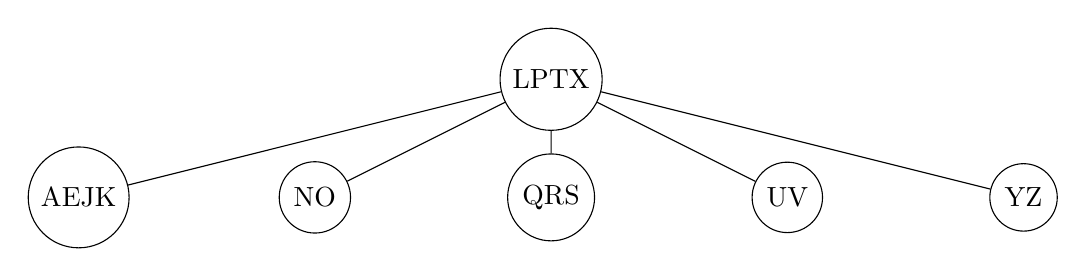
\begin{tikzpicture}[level/.style={sibling distance=30mm/#1}]
\node [circle,draw] (a){LPTX}
  child {
  node [circle,draw] (b) {AEJK}
  }
  child {
  node [circle,draw] (c) {NO}
  }  child {
  node [circle,draw] (d) {QRS}
  }
  child {
  node [circle,draw] (e) {UV}
  }
  child {
  node [circle,draw] (f) {YZ}
  };
\end{tikzpicture}

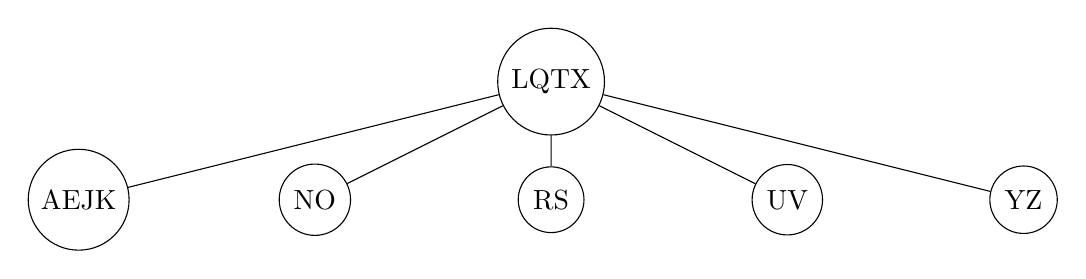
\begin{tikzpicture}[level/.style={sibling distance=30mm/#1}]
\node [circle,draw] (a){LQTX}
  child {
  node [circle,draw] (b) {AEJK}
  }
  child {
  node [circle,draw] (c) {NO}
  }  child {
  node [circle,draw] (d) {RS}
  }
  child {
  node [circle,draw] (e) {UV}
  }
  child {
  node [circle,draw] (f) {YZ}
  };
\end{tikzpicture}

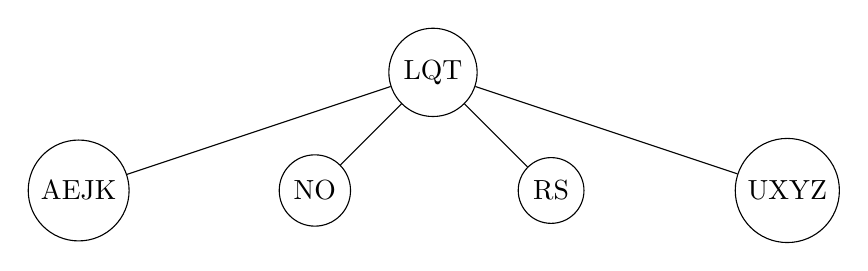
\begin{tikzpicture}[level/.style={sibling distance=30mm/#1}]
\node [circle,draw] (a){LQT}
  child {
  node [circle,draw] (b) {AEJK}
  }
  child {
  node [circle,draw] (c) {NO}
  }  child {
  node [circle,draw] (d) {RS}
  }
  child {
  node [circle,draw] (e) {UXYZ}
  }
;
\end{tikzpicture}



\noindent\textbf{Problem 18-1}\\
\begin{enumerate}[a.]
\item
We will have to make a disk access for each stack operation. Since each of these disk operations takes time $\Theta(m)$, the CPU time is $\Theta(mn)$.

\item
Since only every $m$th push starts a new page, the number of disk operations is approximately $n/m$, and the CPU runtime is $\Theta(n)$, since both the cotribution from the cost of the disk access and the actual running of the push operations are both $\Theta(n)$.
\item
If we make a sequence of pushes until it just spills over onto the second page, then alternate popping and pulling many times, the asymptotic number of disk accesses and CPU time is of the same order as in part a. This is because when we are doing that alternating of pops and pushes, each one triggers a disk access.
\item
We define the potential of the stack to be the absolute value of the difference between the current size of the stack and the most recently passed multiple of $m$. This potential function means that the initial stack which has size 0, is also a muiltiple of $m$, so the poential is zero. Also, as we do a stack operation we either increase or decrease the potential by one. For us to have to load a new page from disk and write an old one to disk, we would need to be at least $m$ positions away from the most recently visited multiple of $m$, because we would have had to just cross a page boundary. This cost of loading and storing a page takes (real) cpu time of $\Theta(m)$. However, we just had a drop in the potential function of order $\Theta(m)$. So, the ammortized cost of this operation is $O(1)$.

\end{enumerate}

\end{document}